%###################################################################################################
\section{Introduction}

\textbf{Properties of Multicellular Systems}
\begin{enumerate}
    \item Stochastic -> Irreversible
    \item Dissipative (take up energy, non-equilibrium, decrease entropy)
\end{enumerate}

Over the course of the last decades, many \acp{cabm} have been proposed and
implemented~\cite{Pleyer2023}.
Their puposes range from early embryogenesis to cancer research over to wound
healing~\cite{Ziraldo2013}.
Some of these models provide exact mathematical formulations \cite{Ghaffarizadeh2018,Tanaka2015} of
the system which they solve.
Although it is well-known that \acp{abm} and \acp{ca} are a subclass of (continous or discrete)
dynamical systems \cite{Wolfram1984} so far \acp{ca} have been studied mathematically to great
extent while \acp{cabm} remain largely untouched on a conceptual level.
We aim to provide insights into a variety of shared concepts among many \acp{cabm} and explain them
along specific examples with real use-cases.
We construct this formalism with the same thought processes that lead to the creation of our
numerical simulation framework \lstinline{cellular_raza}~\cite{Pleyer_cellular_raza_2024}.

\acp{abm} are centered around the thought that cells are the fundamental building-blocks of nature.
Every cellular agent must be assumed to be distinct to any other and can in principle (although hard
in practice) be traced throughout space and time.\todo{CITATION}
The combined individual behaviours of many cells can result in the emergence of global phenomena
such as spatial or temporal patterns \cite{Owen2020,Wolpert1969,Giudicelli2007}.

\begin{itemize}
    \item (C) Cellular Processes
    \item (CC) Cell-Cell Interactions
    \item (DC) Domain-Cell Interactions
\end{itemize}

The cells live within the physical domain and may interact with it in various ways eg. via exchange
of nutrients or via physical forces.
Furthermore, cells can interact with each other directly.
Most of these interactions are of short range compared to the total size of the system although
counter-examples such as electrical signals exist \cite{Ded2021}.

\begin{itemize}
    \item Local interactions
    \item Same as Neighborhoods in \acp{ca}
\end{itemize}

\todo{maybe insert this later?}
We explicitly note that our assumptions are not fundamental and loosening of these restrictions can
be discussed to possibly cover a wider variety of problems.
It is important to consider these limitations when applying this theoretical framework.

\begin{itemize}
    \item What has been done so far?
    \item List cellular \acp{abm} and say which have some mathematical support
    \item List papers of applications with explicit mathematical formulations
    \item Discuss which of the application papers are "implementations" of the abstract frameworks
\end{itemize}

\begin{table}[h]
    \centering
    \begin{tabular}{lccc}
        \toprule
        \acs{abm} & \makecell[c]{Mathematical\\ Formulation} & \makecell{Individual-\\ Based} & Extensibility\\
        \midrule
        Biocellion~\cite{Kang2014} & \cross & \checkmark &\\
        BSim~\cite{Gorochowski2012} & ? & \checkmark &\\
        Chaste (cell-based)~\cite{Cooper2020} & \checkmark & \checkmark &\\
        CompuCell3D~\cite{Swat2012} & \checkmark & \cross \\
        EPISIM~\cite{Aghaallaei2021} \\
        Morpheus~\cite{Starru2014} & ? & (\checkmark) & ?\\
        MultiCellSim~\cite{Dang2020}\\
        PhysiCell~\cite{Ghaffarizadeh2018} & \checkmark & \checkmark & \\
        TSim/CellSys~\cite{Hoehme2010}\\
        VirtualLeaf~\cite{Merks2011}\\
        \bottomrule
    \end{tabular}
    \caption{
        Various \acp{abm} and their mathematical descriptiveness.
        \todo{make better}
    }
\end{table}

%###################################################################################################
\section{Mathematical Foundations}
%---------------------------------------------------------------------------------------------------
\subsection{The Cellular Space $\mathscr{C}$}
This section aims to construct a space in which individual cells can be represented.
We construct these notions purely from known biological behavioural principles.
By formulating these concepts in abstract mathematical terms, we allow ourselves to cover a wide
variety of \acp{abm}.
It is clear that this approach targets models on the mesoscopic scale such that not every
fundamental effect can be taken into account.

We assume that each individual cell lives in a set $C$ which describes all possible configurations
of this single cell.
Cellular systems are characterized by the fact that cells are in principle (although in
practice sometimes more difficult) tracable through time and space.
Depending on the cellular representation we might encounter two cells with identical parameters and
properties (eg. position, intracellular concentrations) which are still distinct agents and can not
be interchanged arbitrarily.
This case could occur eg. when representing cellular positions by whole numbers as in a
\ac{ca}.
This point is further made clear when thinking about cellular proliferation as a tree.
Figure~\ref{fig:cell-lineage-break} shows a hypothetical change between two child-cells.
If we would interchange child $c_{12}$ with $c_{21}$, this would mean that two grandchild-cells
$gc_{212}$ and $gc_{221}$ would have different grandparent-cells.

\begin{figure}[h]
    \centering
    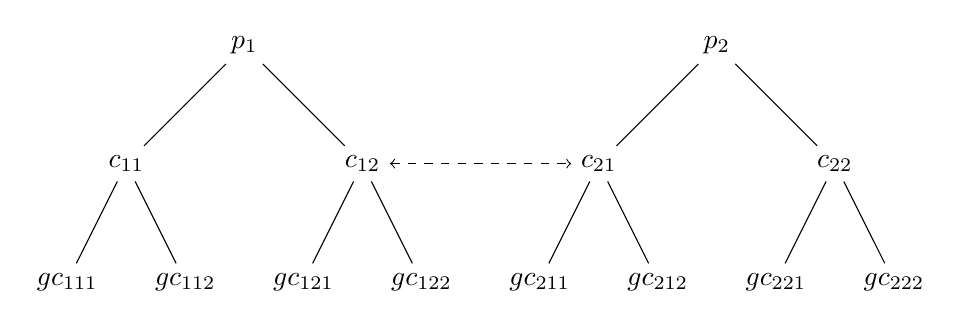
\begin{tikzpicture}[level distance=1.5cm,
        level 1/.style={sibling distance=3cm},
        level 2/.style={sibling distance=1.5cm}
    ]
        \node (p1) {$p_1$}
            child {node (c11) {$c_{11}$}
                child {node (gc111) {$gc_{111}$}}
                child {node (gc112) {$gc_{112}$}}
            }
            child {node (c12) {$c_{12}$}
                child {node (gc121) {$gc_{121}$}}
                child {node (gc122) {$gc_{122}$}}
            };
        \node[] at (6, 0) {$p_2$}
            child {node (c21) {$c_{21}$}
                child {node (gc211) {$gc_{211}$}}
                child {node (gc212) {$gc_{212}$}}
            }
            child {node {$c_{22}$}
                child {node (gc221) {$gc_{221}$}}
                child {node (gc222) {$gc_{222}$}}
            };
        \draw[dashed,<->] (c12) -- (c21);
        \end{tikzpicture}
        \caption{
            Arbitrary cells can not be interchanged freely since this might introduce incorrect
            configurations into the cell-lineage.
            For example, the two cousin-cells $gc_{212}$ and $gc_{221}$ would have different
            grandparent-cells if $c_{12}$ and $c_{21}$ would be interchanged.
        }
        \label{fig:cell-lineage-break}
\end{figure}

This exemplifies the need to assign unique identifiers for cells to correctly trace their lineage.
We call the set of all identifiers $J$ and only consider cells as a combination of an element
$c\in C$ with an identifier $\iota\in I$.
Thus a cell is an element of the product $J\times C$.
The explicit representation of $J$ can depend on the respective system in question.
To allow for processes such as cell-division and death we additionally must be able to treat a
variable number of cells throughout the evolution of the dynamical system.
The evolution function of our dynamical system will map cellular states onto each other, thus
acting on the cellular space $\mathscr{C}$.
As can be seen from Figure~\ref{fig:cell-lineage-break}, division of cells introduces two new
identifiers for two new cells and consumes the previously existing cell.
Cell-death removes cells.
Newly inserted cells may not obtain previously used identifiers since this would again interfere
with cell lineage.
This means, we need to keep track of all identifiers $\iota\in I_p$ which have been used in the
past.

\begin{definition}[Cellular State]
    \label{def:cellular-state}
    Let $I$ be a set of identifiers and $C$ be the set describing cellular agents.
    We call a set of cells $(I_p,M)\in Pot(I)\times Pot(I\times C)$ a cellular state if
    \begin{enumerate}
        \item Every cell has a unique identifer $\#\pi_1(M)=\#M$.
        \item Identifiers have not been used previously $I_p\cap\pi_1(M)=\emptyset$
    \end{enumerate}
    where $\pi$ is the projection on the first component.
    The set $I_p$ contains identifiers which have been used previously.
\end{definition}

\begin{definition}[Cellular Space]
    \label{def:cellular-space}
    The cellular space $\mathscr{C}(I, C)$ of an index set $I$ and cellular configuration space $C$
    is given by
    $\mathscr{C}(I,C) = \{M\in Pot(I)\times Pot(I\times C) | M \text{ is cellular state }\}$.
    We may choose the simplified notation $\mathscr{C} = \mathscr{C}(I, C)$ where the context is
    clear.
    We write $c_\iota:=(\iota,c)\in M$ where $(I_p,M)\in\mathscr{C}$ despite the non-exhaustiveness
    of the index $\iota$ in a single cellular state.
\end{definition}

Cell division~\cite{bhlitem268752} is a process during which a cell transforms either via binary
(or multiple) fission~\cite{Biov2014} or mitosis~\cite{Ilowiecki1981,von1835resp} and
meiosis~\todo{CITATION} into separate
daughter cells.
To describe cell division, the dynamics behind this transition needs to be taken into account.
We will discuss this in the chapter~\ref{section:dynamics}.
In our agent-based approach, the end of this transition removes the old cell and inserts the new
daughter cells.

\begin{definition}[Single Cell Division]
    \label{definition:cell-division-single}
    We call a map $\gamma:C\rightarrow \cup_{n\geq 2}C^n$ a single division function and
    $\Upsilon:\{\gamma:C\rightarrow \cup_{n\geq 2}C^n\}\times I\times\mathscr{C}\rightarrow\mathscr{C}$ a 
    single division operator if for any initial state $(I_p,M)\in\mathscr{C}$ with $d_i\in M$ and
    final state $(J_p,N)=\Upsilon(\eta,i,(I_p,M))$
    \begin{enumerate}
        \item (Removal) Exactly one cell is removed $M\backslash N=\{d_i\}$
        \item (Insertion) At least two new cells are created:
            $N\backslash M=\{c_\iota,\tilde{c}_{\tilde{\iota},\dots}\}$
        \item (Tracking) We carry forward all old identifiers and the removed one: $J_p=I_p\cup\{i\}$
        \item (Uniqueness) New cells have new identifiers: $\iota,\tilde{\iota},\dots\notin J_p$.
    \end{enumerate}
    In the case when $i\notin\pi_1(M)$, we require $\Upsilon(\eta,i,(I_p,M))=(I_p,M)$.
    The last two conditions are to be thought of as one in order to guarantee uniqueness for each
    cell over the course of the total time of our system.
\end{definition}

\begin{definition}[Cell Division]
    \label{definition:cell-division}
    A division function $\gamma$ is the concatenation of single division functions
    $\{\gamma_i,i\in I\}$.
    We require that the overall effect is independent of the order of their individual applications,
    ie.
    \begin{equation}
        \prod\limits_{i_j\in I}\gamma_{i_j} = \prod\limits_{i\in I}\gamma_i
    \end{equation}
    where the product is with respect to the concatenation of maps.
\end{definition}

It is important to note that while this definition seems cumbersome in the first place, it is
essential in upkeeping a valid cellular state.
From an application standpoint, it is desirable to only specify the division map $\gamma$ and have
$\Upsilon$ be defined by the underlying modeling framework.

Another important process is that of cell death which is similarly as cell-division not instantanous
but occurs over a period of time.
Death schemes are categoritzed into programmed cell-death, also known as apoptosis~\cite{Kerr1965}
and necrosis~\cite{Gerschenson2001} which occurrs due to damage from external effects.
In principle, these processes take time in order to commence and the cell may interact with its
environment (ie. through secretion) during this stage.
Such transitions can be described by \todo{fill this} and will be discussed in
chapter~\ref{section:dynamics}.
Once the process of dying is over, the cell is removed.

\begin{definition}[Cell Death]
    \label{definition:cell-death}
    % We call a map $\zeta:I_p\rightarrow \text{Pot}(I_p)$ a death-function
    Any cell-death removes a particular index $\iota\in I_p$.
    Thus the combination of many cell-daths is a mapping $\zeta:I_p\rightarrow \text{Pot}(I_p)$
    where $\text{Pot}(I_p)$ is the power set of $I_p$.

\todo{
    - apoptosis
    - necrosis
    - removal
}
\end{definition}

\begin{lemma}[Cell Lineage]
    \label{lemma:cell-lineage}
    Given an initial state $(I_p,M)\in\mathscr{C}$, an arbitrary combination of applications of
    division and death functions creates a forest.
\end{lemma}
\begin{proof}
    We proof this statement via induction. For $n=0$ we are presented with a cellular state
    $M\in\mathscr{C}$ which consists of cells $\{c_\iota\in M\}$.
    We interpret each cell as root of a new tree.
    In the induction step $n\rightarrow n+1$, we may assume that $G=(C,E)$ is a tree with
    cells as vertices.
    Any application of a division function $\Upsilon(\gamma, \dot)$ consumes a cell $c_{\iota_0}$
    and produces new cells $\{c_{\iota_1},\dots,c_{\iota_n}\}$.
    We thus insert the new cells as additional vertices with the edges
    $\{c_{\iota_0},c_{\iota_1}\},\dots,\{c_{\iota_0},c_{\iota_n}\}$.
    From the Uniqueness property of the cell-division definition~\ref{definition:cell-division},
    we know that the index of the removed cell $c_{\iota_0}$ will not occur for any further
    application of the division operator which means that the vertex of cell $c_{\iota_0}$ has $n$
    children.
    In the case of a death function, nothing happens.
    The associated cell $c_\iota$ will remain and endpoint for any further applications of death
    or division.
\end{proof}
\begin{corollary}[$k$-ary and Binary Cell Division]
    In the case where the single division function
    $\eta:C\rightarrow C^k\subset\cup_{n\in\mathbb{N}}C^n$
    is of k-ary nature, lemma~\ref{lemma:cell-lineage} retains a k-ary tree.
    The most common biological reality is the binary case.
\end{corollary}

%###################################################################################################
\subsection{Dynamics}
\label{section:dynamics}
\begin{definition}[Dynamical System]
    A dynamical system is a tuple $(T,M,\phi)$ where $T$ is a monoid (written additively) and
    $\phi$ is a mapping
    \begin{equation}
        \phi : U\subset(T\times M) \rightarrow M
    \end{equation}
    with $\pi_2(U) = M$ where $\pi_2$ is the projection on the second coordinate and $\phi$
    satisfies
    \begin{align}
        \phi(0,m) &= m\\
        \phi(t_2, \phi(t_1, m)) &= \phi(t_2+t_1,m).
    \end{align}
\end{definition}

We often write $\phi(t,m) = \phi_t(m)$.
The dynamics of \acp{abm} are governed by agents and their interactions with each other and the
simulation domain.
Thus we define our dynamical system to be of this shape.

\begin{definition}
    An \ac{abm} is a dynamical system which consists of a Cellular Space $\mathscr{C}$ and a domain
    $\mathscr{D}$.
    \begin{equation}
        M = \mathscr{C}\times\mathscr{D}
    \end{equation}
    Given an initial state $x_0$, we say that a cell $c$ with index $\iota$ is alive at point $t$ if
    $c_\iota\in\pi_1(\phi_t(x))$.
\end{definition}

It is of importance to consider the domain as part of the dynamical system such that interactions
of the agents with it can permanently alter its constitution.
In this way, extracellular constituents can interact and change and even the overall morphology of
the domain could be affected by dynamics and interactions.

\todo{Define our dynamical system more precisely. What does it mean to be an index?
$\iota\in\phi_t$}

\begin{lemma}[Cellular Identity]
    \label{thm:cellular-uniqueness}
    Given an index $\iota\in I$ to an initial state $x$ of an \ac{abm}, we define the
    \textbf{Life-Span} of $\iota$ which is the set of all time-points for which the cell is alive
    \begin{equation}
        T_\iota=\{t\in T: c_\iota \text{ is alive}\}.
    \end{equation}
    If $T$ be a ordered and path-connected topological space, then $T_\iota$ is also path-connected.
    If $\mu$ is a measure on $T$, we also define the \textbf{Lifetime} with respect to this measure
    via
    \begin{equation}
        t_\iota:=\mu\left(T_\iota\right).
    \end{equation}
    In practial examples, $\mu$ will be given by the Lebesgue measure.
\end{lemma}
\begin{proof}
    Let $t<s\in T_\iota$ arbitrary.
    We pick a path $\gamma:[0,1]\rightarrow T$ from $t$ to $s$.
    Since $T$ is ordered, we can pick a path which satisfies $t\leq\gamma(h)\leq s$.
    By Definition~\ref{definition:cell-division}, properties 1 and 4, we see that every state
    between the points of insertion and removal are part of $T_\iota$ and thus
    $\gamma(h)\in T_\iota\forall h\in [0,1]$.
\end{proof}

\begin{corollary}
    If $T=\R$
\end{corollary}

\todo{practial implementations of Index choosing}
\begin{enumerate}
    \item Assign via voxel and counting
    \item Assign via parent
\end{enumerate}

% ..................................................................................................
\subsubsection{Spatial Locality}
We assume that the physical domain $D$ can be split into smaller subdomains
$\bigcup_{i\in I}S_i=D$ which are pairwise disjoint.
We will later require that any dynamics can be calculated by considering cellular agents inside a
given subdomain $S_i$ and their interactions with neighboring subdomains.
This also applies to spatial effects such as diffusion.
Therefore, we must first develop the notion of being a \textbf{neighbor}.

\begin{definition}[Neighbor]
    The notion of neighbor can be defined by two equivalent methods.
    \begin{enumerate}
        \item We call $\eta:I\rightarrow Pot(I)$ a \textbf{neighbor map} if
        \item $i\in\eta(j) \Leftrightarrow j\in\eta(i)$ for each $i,j\in I$.
            We call a relation $||$ on $I$ a \textbf{neighbor relation} if it is symmetric.
    \end{enumerate}
\end{definition}

\begin{example}[Moore Neighbors]
    The neighborhood used in the Game of Life~\ref{example:game-of-life} is the 2-dimensional
    special case.
    In general, for any discrete space $\mathbb{Z}^n$, we consider the Moore neighborhood $U(x)$ for
    any point $x\in\mathbb{Z}^n$ to be
    \begin{equation}
        U(x) := \{y\in\mathbb{Z}^n:\max\limits_{i\in\{1..n\}}|x_i-y_i|=1\}.
    \end{equation}
    This definition ensures that at least one component of the value $y$ is not identical to the
    point in question $x$.
    This metric is also often called uniform norm, supremum norm (in a possibly infinite-dimensional
    case) or Chebyshev norm~\cite{Rudin1976}.
\end{example}

Note that in the numerical implementation it is often more convenient to work with the first
definition while the second can be more useful in a theoretical context.

\begin{proof}
    $1) \Rightarrow 2)$ Let $\eta$ be a neighbor map.
    We define a relation $||$ by $i||j \Leftrightarrow i\in\eta(j)$.
    It is clear that $||$ is symmetric.\\
    $2) \Rightarrow 1)$ Let $||$ be a symmetric relation on $I$.
    We define the function $\eta:I\rightarrow Pot(I)$ via
    $\eta(i):=\{j\in I \text{ such that } i||j\}$.
    If $j\in\eta(i)$ then $i||j \Leftrightarrow j||i$ and thus $i\in\eta(j)$.
\end{proof}

Equipped with this notion of \textbf{neighbor}, we can now formalize the spatial splitting of our
domain.

\begin{definition}[Spatial Decomposition]
    A Spatial Decomposition of a domain $D$ is a collection of subsets
    $\{S_i\subset D: i\in I\}$ together with a either a neighbor map $\eta$ or neighbor relation
    $||$ such that $D=\cup_{i\in I}$ and $S_i$ are pairwise disjoint.
\end{definition}
\input{cellular-aspects}

\subsection{Comparison with \aclp{ca}}
\label{section:comparison-with-ca}
Classical \acp{ca} such as Conway's Game of Life \cite{games1970fantastic} \todo{MORE CITATIONS}
% or the Cellular Potts Model \cite{Graner1992}
are spatially and temporally discrete dynamical systems.
\todo{More details about \acp{ca}}
\todo{Cells are not tracable through time and space}
\todo{division and death}
\todo{distinction to migration not clear}
In the case of \acp{abm} the space $M$ consists of the collection of all currently living cells
$\mathscr{C}$ and the physical domain $D$ in which they live ie. $M=\mathscr{C}\times D$.

\begin{example}[Game of Life]
    \label{example:game-of-life}
    Conway's Game of Life is perhaps the most popular example for a cellular automaton.
    It is deterministic and acts on a infinite grid $\mathbb{Z}^2$ by assigning one of two states
    (alive or dead) to each grid-point
    \begin{equation}
        L:\mathbb{Z}^2\rightarrow\{0,1\}
    \end{equation}
    where we prefer the short-hand notation $L(i,j)=L_{ij}$ or $L^n_{ij}$ where $n$ is the temporal
    index.
    This means a single state is described by a mapping $L:\mathbb{Z}^2\rightarrow\{0,1\}$ and the
    evolution function of this dynamical system acts on the space of these maps
    $X:=\{L:\mathbb{Z}^2\rightarrow\{0,1\}\}$
    \begin{equation}
        \phi:U\subset(\mathbb{N}\times X) \rightarrow X
    \end{equation}
    where we identified $(\mathbb{N},+)$ as the monoid of the dynamical system.
    Let $\eta_{ij}\subset\mathbb{Z}^2$ be the set of spatial indices which are direct neighbors of
    $(i,j)$ ie. $\eta_{ij}=\{(k,l)\in\mathbb{Z}^2 \text{ where } |k-i|<2, |l-j|<2 \text{ and }
    (k,l)\neq(i,j)\}$.
    The game consists of three rules:
    \begin{enumerate}
        \item Any live cell with fewer than two live neighbors dies, as if by underpopulation.
        \item Any live cell with two or three live neighbors lives on to the next generation.
        \item Any live cell with more than three live neighbors dies, as if by overpopulation.
        \item Any dead cell with exactly three live neighbors becomes a live cell, as if by
            reproduction.
    \end{enumerate}
    Together with the sum of all neighboring cells $S_{ij}=\sum\limits_{\iota\in\eta_{ij}}L^n_\iota$
    we can write these as
    \begin{equation}
        \phi_1(L_{ij}^n) = L_{ij}^{n+1} =
        \begin{cases}
            0 &L^n_{ij}=1 \text{ and } S_{ij}<2\\
            1 &L^n_{ij}=1 \text{ and } S_{ij}=2,3\\
            0 &L^n_{ij}=1 \text{ and } S_{ij}>3\\
            1 &L^n_{ij}=0 \text{ and } S_{ij}=3\\
            0 &\text{else}
        \end{cases}
    \end{equation}
    which fully specifies the dynamical system when applying iteratively
    $\phi_m=\phi_1\circ\dots\circ\phi_1$.
\end{example}

When we compare the above rules with definitions~\ref{def:cellular-state}
and~\ref{def:cellular-space}, we immediately see that the cellular identity is not preserved for the
4th rule.
This \ac{ca} assumes that a new cell is created from 3 neighboring cells which is contrary to the
division process of cells.
We set out to formualte the Game of Life within the framework of cellular \acp{abm}.
To circumvent this problem, we could assume that simply one of the present cells divides and is
chosen randomly with even probability.
In order to formalize such a system we would require to introduce the notion of a
Stochastic Dynamical System.
But this raises the problem that the second cell of this division process would have to also be
inserted somewhere in the \ac{ca}.
Asked in more general terms: Given an arbitrary state $L^n_{ij}$:
Is it possible to describe a single transition $L^n_{ij}\rightarrow L^{n+1}_{ij}$ by a combination
of finitely many cellular division and death processes?
In general: No.
This is made clear by considering the example of Figure~\ref{fig:conway-non-abm-transition}.
The transition shown can not be described by any combination of division and death under the
consideration that cell-death can only act on currently alive cells.
In principle, this conundrum could be lifted when performing the division and death process in
different steps but this would change the outcome and behaviour of the system.
Similarly, other \acp{ca} such as the Cellular Potts Model~\cite{Graner1992} or Rule
184~\cite{Krug1988} can not
directly be translated into an \ac{cabm}.
This shows that even the fundamental choices in the design of \acp{cabm} already present interesting
restrictions and \acp{ca} should in general not be treated as special cases of \acp{cabm} but as
distinct entities.

\begin{figure}[h]
    \centering
    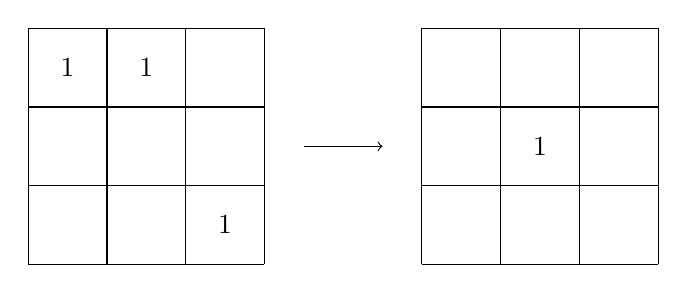
\begin{tikzpicture}
        \draw (0,0) -- (3,0);
        \draw (0,0) -- (0,3);
        \draw (3,0) -- (3,3);
        \draw (0,3) -- (3,3);
        \draw (1,0) -- (1,3);
        \draw (2,0) -- (2,3);
        \draw (0,1) -- (3,1);
        \draw (0,2) -- (3,2);
        \node at (2.5,0.5) {1};
        \node at (0.5,2.5) {1};
        \node at (1.5,2.5) {1};
        \draw[->] (3.5,1.5) -- (4.5,1.5);
        \draw (0+5,0) -- (3+5,0);
        \draw (0+5,0) -- (0+5,3);
        \draw (3+5,0) -- (3+5,3);
        \draw (0+5,3) -- (3+5,3);
        \draw (1+5,0) -- (1+5,3);
        \draw (2+5,0) -- (2+5,3);
        \draw (0+5,1) -- (3+5,1);
        \draw (0+5,2) -- (3+5,2);
        \node at (1.5+5,1.5) {1};
    \end{tikzpicture}
    \caption{
        This transition in Conways Game of Life can not be described by any combination of
        cell-division and death.
        The cell in the middle which is being created by rule 4 is new and must thus be created by
        the division mechanism in our \ac{abm}.
        If any of the initial cells divide, we obtain 2 new cells which need to placed.
        Since cell-death can only affect currently existing cells, this is contradictory to the
        final state which only contains a single cell.
    }
    \label{fig:conway-non-abm-transition}
\end{figure}

This statement can be generalized to the class of elementary \acp{ca}~\cite{Wolfram1983}.
The statement of the following theorem relies on a number of assumptions.
We assume that during the advancement of the \ac{ca} only one of two processes is triggered:
division or death.
The particular reason for any one of them is not taken into account as this depends on which
problem is being modeled.
We explicitly exclude other processes such as stochastic effects and spatial movement
(compare Table~\ref{tab:cellular-aspects}).

\begin{theorem}[Elementary \aclp{ca} are not cell-based]
    Elementary \acp{ca} are characterized by their transition rules.
    In total there are $8$ states from which the next value is determined.
    To simplify notation, the Wolfram Code (Figure~\ref{fig:wolfram-code}) was
    proposed~\cite{Wolfram1994-yw}.
    \begin{figure}[h]
        \centering
        \begin{tabular}{ r c c c c c c c c }
            Current State & $111$ & $110$ & $101$ & $100$ & $011$ & $010$ & $001$ & $000$\\
            \midrule
            New State & $a_8$ & $a_7$ & $a_6$ & $a_5$ & $a_4$ & $a_3$ & $a_2$ & $a_1$\\
            % Reduced     & $a_8$ & $b$   & $a_6$ & $c$   & $b$   & $a_3$ & $c$   & $0$
        \end{tabular}
        \caption{
            Elementary \acp{ca} can be characterized by their transition rules.
            The binary number $a_8\dots a_1$ converted to decimal, results in the rule number of
            the associated \ac{ca} (i.e. $01101110_2=110_d$).
            There exist $256$ rules in total.
        }
        \label{fig:wolfram-code}
    \end{figure}
\end{theorem}
\begin{proof}
    We fist inspect the last transition rule $000\rightarrow a_1$ which presents an empty subspace
    (no cells existing) and advances it.
    If $a_1=1$, we would create a new cell from nothing.
    This is contrary to the biological reality in which cells divide and reproduce.
    We can infer, that \acp{ca} which have $a_1=1$ are not cell-based.
    Furthermore, due to the isotropy of space, we expect that all initial states deliver identical
    results to their mirrored version which requires $a_7=a_4$ and $a_5=a_2$.
    These considerations reduce the total number of possible rules to $2^5=32$.

    \begin{itemize}
        \item Show for all Wolfram Rules that most of them can not be cell-based models
        \item Consider migration as an additional rule instead of just division and death
        \item Formal question: given an initial state $x_0$ and final state $x_1$ does a combination
            of cell-based rules exist which produces this state?
        \item Additional question: Is this procedure deterministic? (It should not have to be
            deterministic imho)
    \end{itemize}
\end{proof}

\paragraph{Scaling Behaviour}

\begin{figure}[h]
    \begin{minipage}{0.45\textwidth}
        \centering
        \begin{tabular}{lccc}
            \toprule
            Growth Type & Dim & Step & Scaling\\
            \midrule
            1D                  & $1$ & $1$ & $2n+1$\\
            2D Moore            & $2$ & $1$ & $(2n+1)^2$\\
            2D von Neumann      & $2$ & $1$ & $2n(n+1)+1$\\
            d-Dim Moore         & $d$ & $1$ & $(2n+1)^d$\\
            d-Dim von Neumann   & $d$ & $1$ & \todo{calculate it}\\
            d-Dim Moore         & $d$ & $k$ & $(2kn+1)^d$\\
            d-Dim von Neumann   & $d$ & $k$ & \todo{calculate it}\\
            \midrule
            Exponential         &     &     & $2^n$\\
            Logistic            &     &     & $\frac{L}{1+e^{-\alpha(n-x_0)}}$\\
            \bottomrule
        \end{tabular}
    \end{minipage}%
    \hspace{0.05\textwidth}%
    \begin{minipage}{0.49\textwidth}
        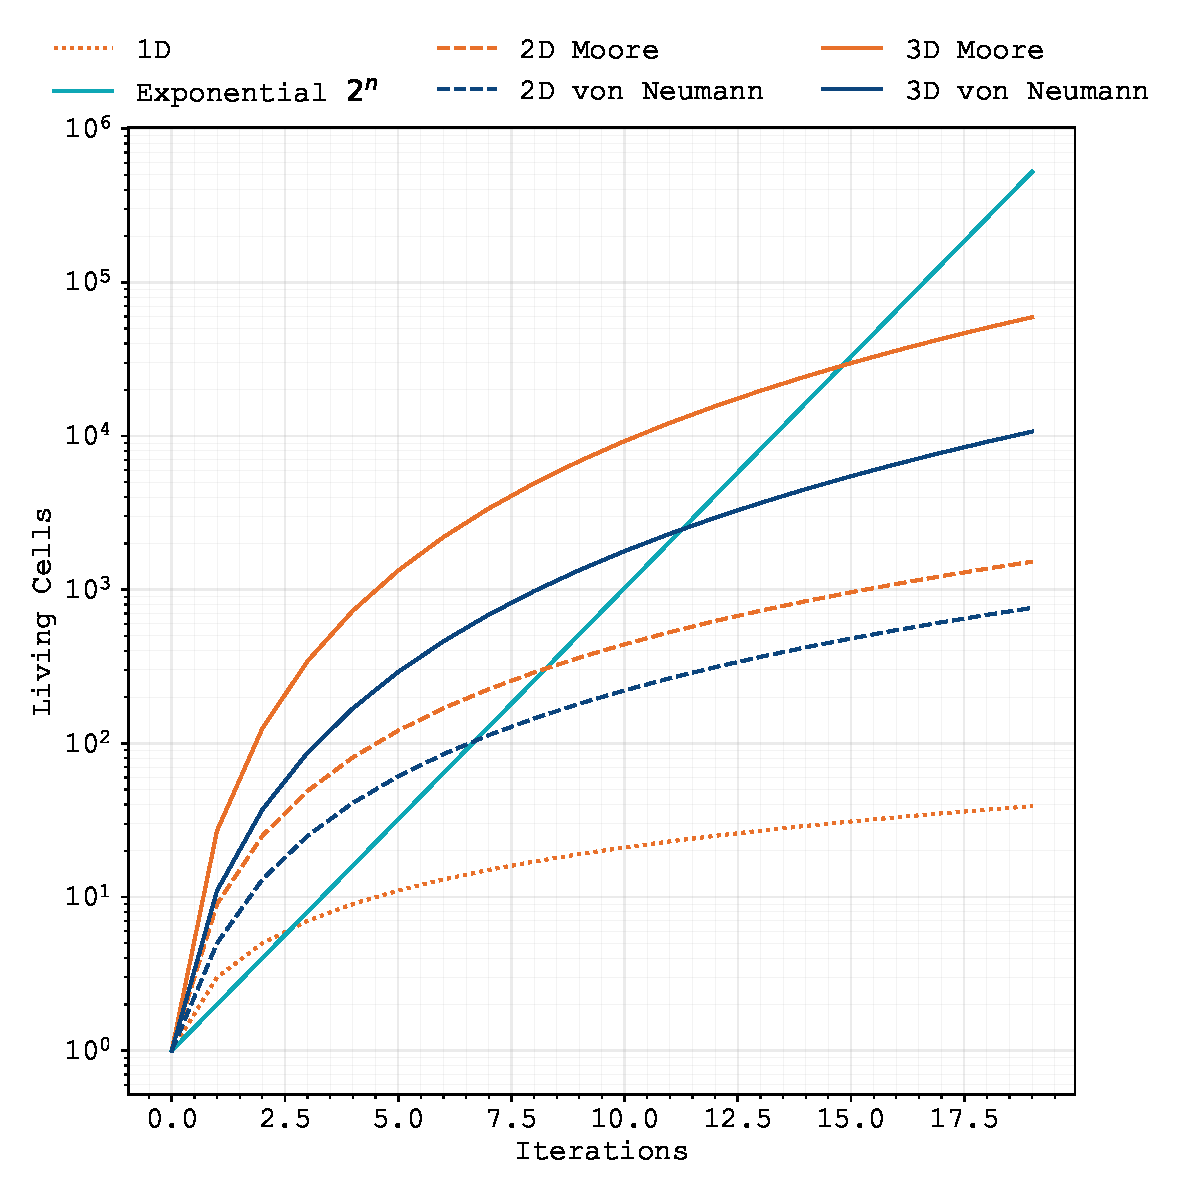
\includegraphics[width=\textwidth]{ca-rules/ca-scaling.pdf}
    \end{minipage}
    \caption{
        Comparison of various scaling rules for different neighborhoods of \acp{ca} and other
        growth curves.
        The graph shows the polynomial nature of \acp{ca} scaling laws compared to the exponential
        nature of either purely exponential or logistic growth.
        The growth parmeter of the logistic growth curve was chosen $\alpha=\log(2)$ in order to
        align with the exponential growth rate of $2^n$.
        The limiting term was chosen $L=3000$ in order to produce visually comparable results and
        $x_0=\log(L-1) / \log(2)$ was chosen such that the initial value is identical to $1$.
    }
    \label{fig:ca-scaling}
\end{figure}

\begin{theorem}[Elementary \acp{ca} cannot describe exponential growth]
\end{theorem}

\begin{itemize}
    \item missing migration aspect
    \item counts only stay local in one "cell"
\end{itemize}
\begin{proof}
\end{proof}

\label{section:applications}


%###################################################################################################
\section{Coarse-Graining Strategies}

\begin{itemize}
    \item \cite{You2018} single-cell model of rod-shaped bacteria, corse-grained model as well
    \item \cite{Wensink2012} \textbf{TODO look at this}
    \item \cite{Peruani2006} \textbf{TODO look at this}
\end{itemize}

%---------------------------------------------------------------------------------------------------
\subsection{Cell Sorting}

\begin{itemize}
    \item Define ratio of spatial density of species 1 and 2 $\rho(x)$
    \item Assume that $\rho(x) = \rho_0\sin(\lambda x)$
    \item Optimize Lagrangian/Hamiltonian with respect to $\lambda$
\end{itemize}

%---------------------------------------------------------------------------------------------------
\subsection{Bacterial Pool Model with Inter-species Competition}

%---------------------------------------------------------------------------------------------------
\subsection{Branching Patterns of \textit{Bacillus Subtilis}}

In our previous work~\cite{Pleyer2025}, we have shown that bacterial branching patterns can be
described by an \ac{abm}

\begin{itemize}
    \item bacterial branching patterns can be modeled by \ac{abm}
    \item list aspects: Mechanics, Interaction, Intracellular \& Extracellular Reactions, Cycle
    \item write down equations
\end{itemize}

\begin{enumerate}
    \item Viewpoint from various scales is inherent for \acp{abm}
    \item Lotka-Volterra Equations: Implement as \ac{abm} and show how to coarse-grain it in order
        to reobtain the desired equations.
    \item Do the same with logistic growth?
    \item Coarse-graining of bacterial-branching: Use multiple agents as one: how do parameters
        change
    \item Compare to Thermodynamics (intensive vs extensive properties, rescaling of system)
    \item Try to formalize it by introducing some type of cutoff $k$ below which we cannot "see"
\end{enumerate}

\begin{figure}[h]
    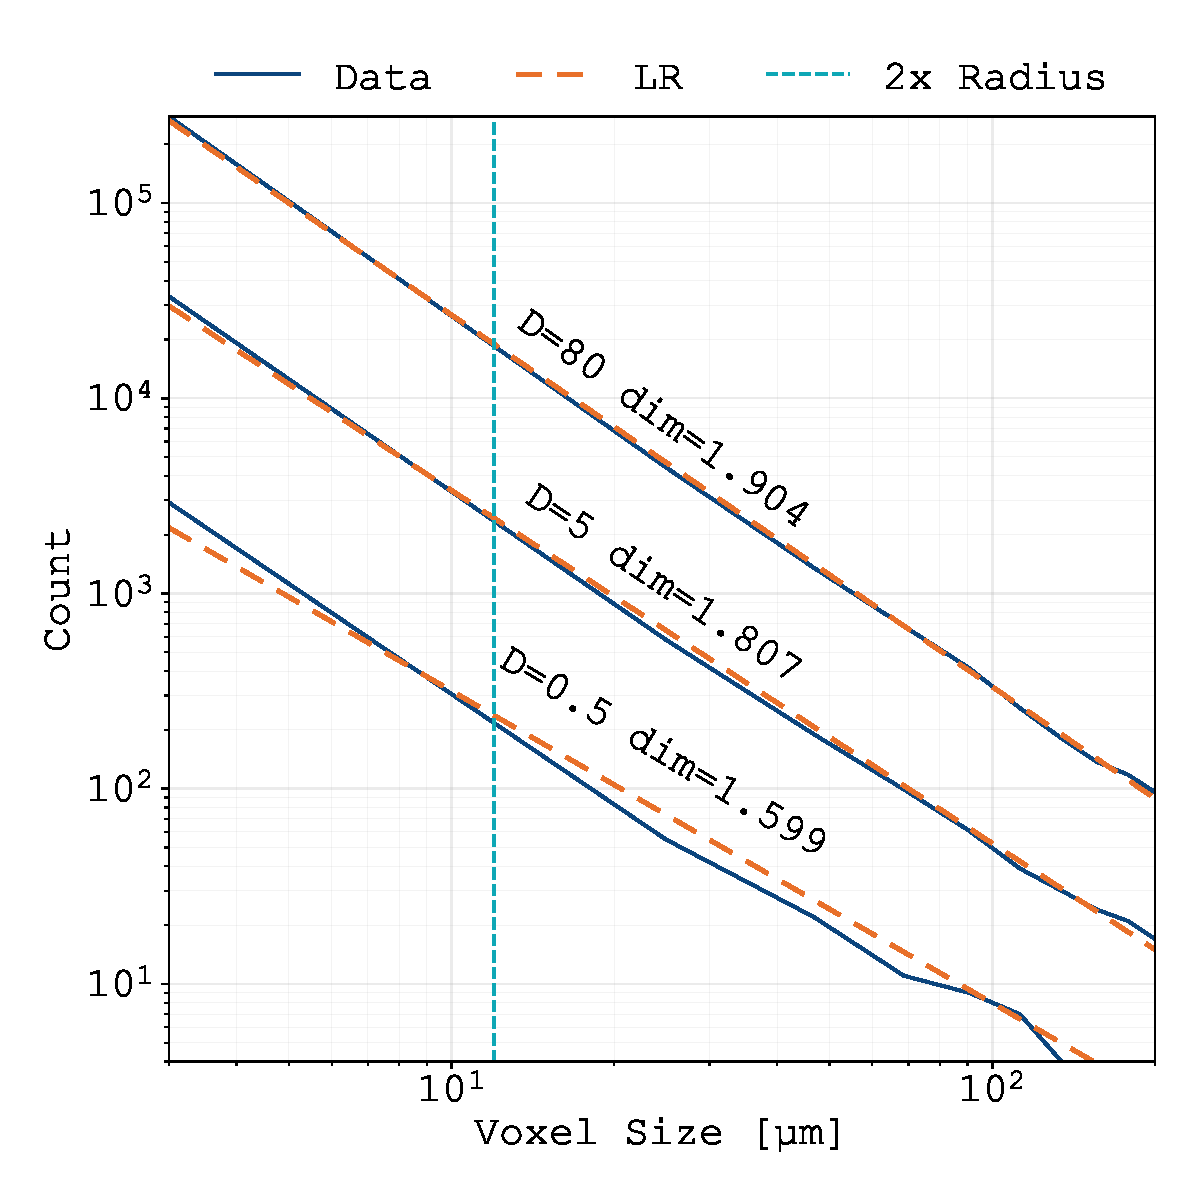
\includegraphics[width=0.5\textwidth]{figures/fractal-dim-box-size-scaling.pdf}%
    \includegraphics[width=0.5\textwidth]{figures/fractal-dim-over-time.pdf}%
    \caption{
        (A) The bacterial branching simulation satisfies the conditions for a self-similar fractal.
        (B) The fractal dimension is not constant in time, but follows a growth curve with upper
        bound.
    }
    \label{fig:bacterial-brancing-fractal-dimension}
\end{figure}

\todo{Think about this}
\url{https://en.wikipedia.org/wiki/Functional_renormalization_group}

\begin{figure}[h]
    \centering
    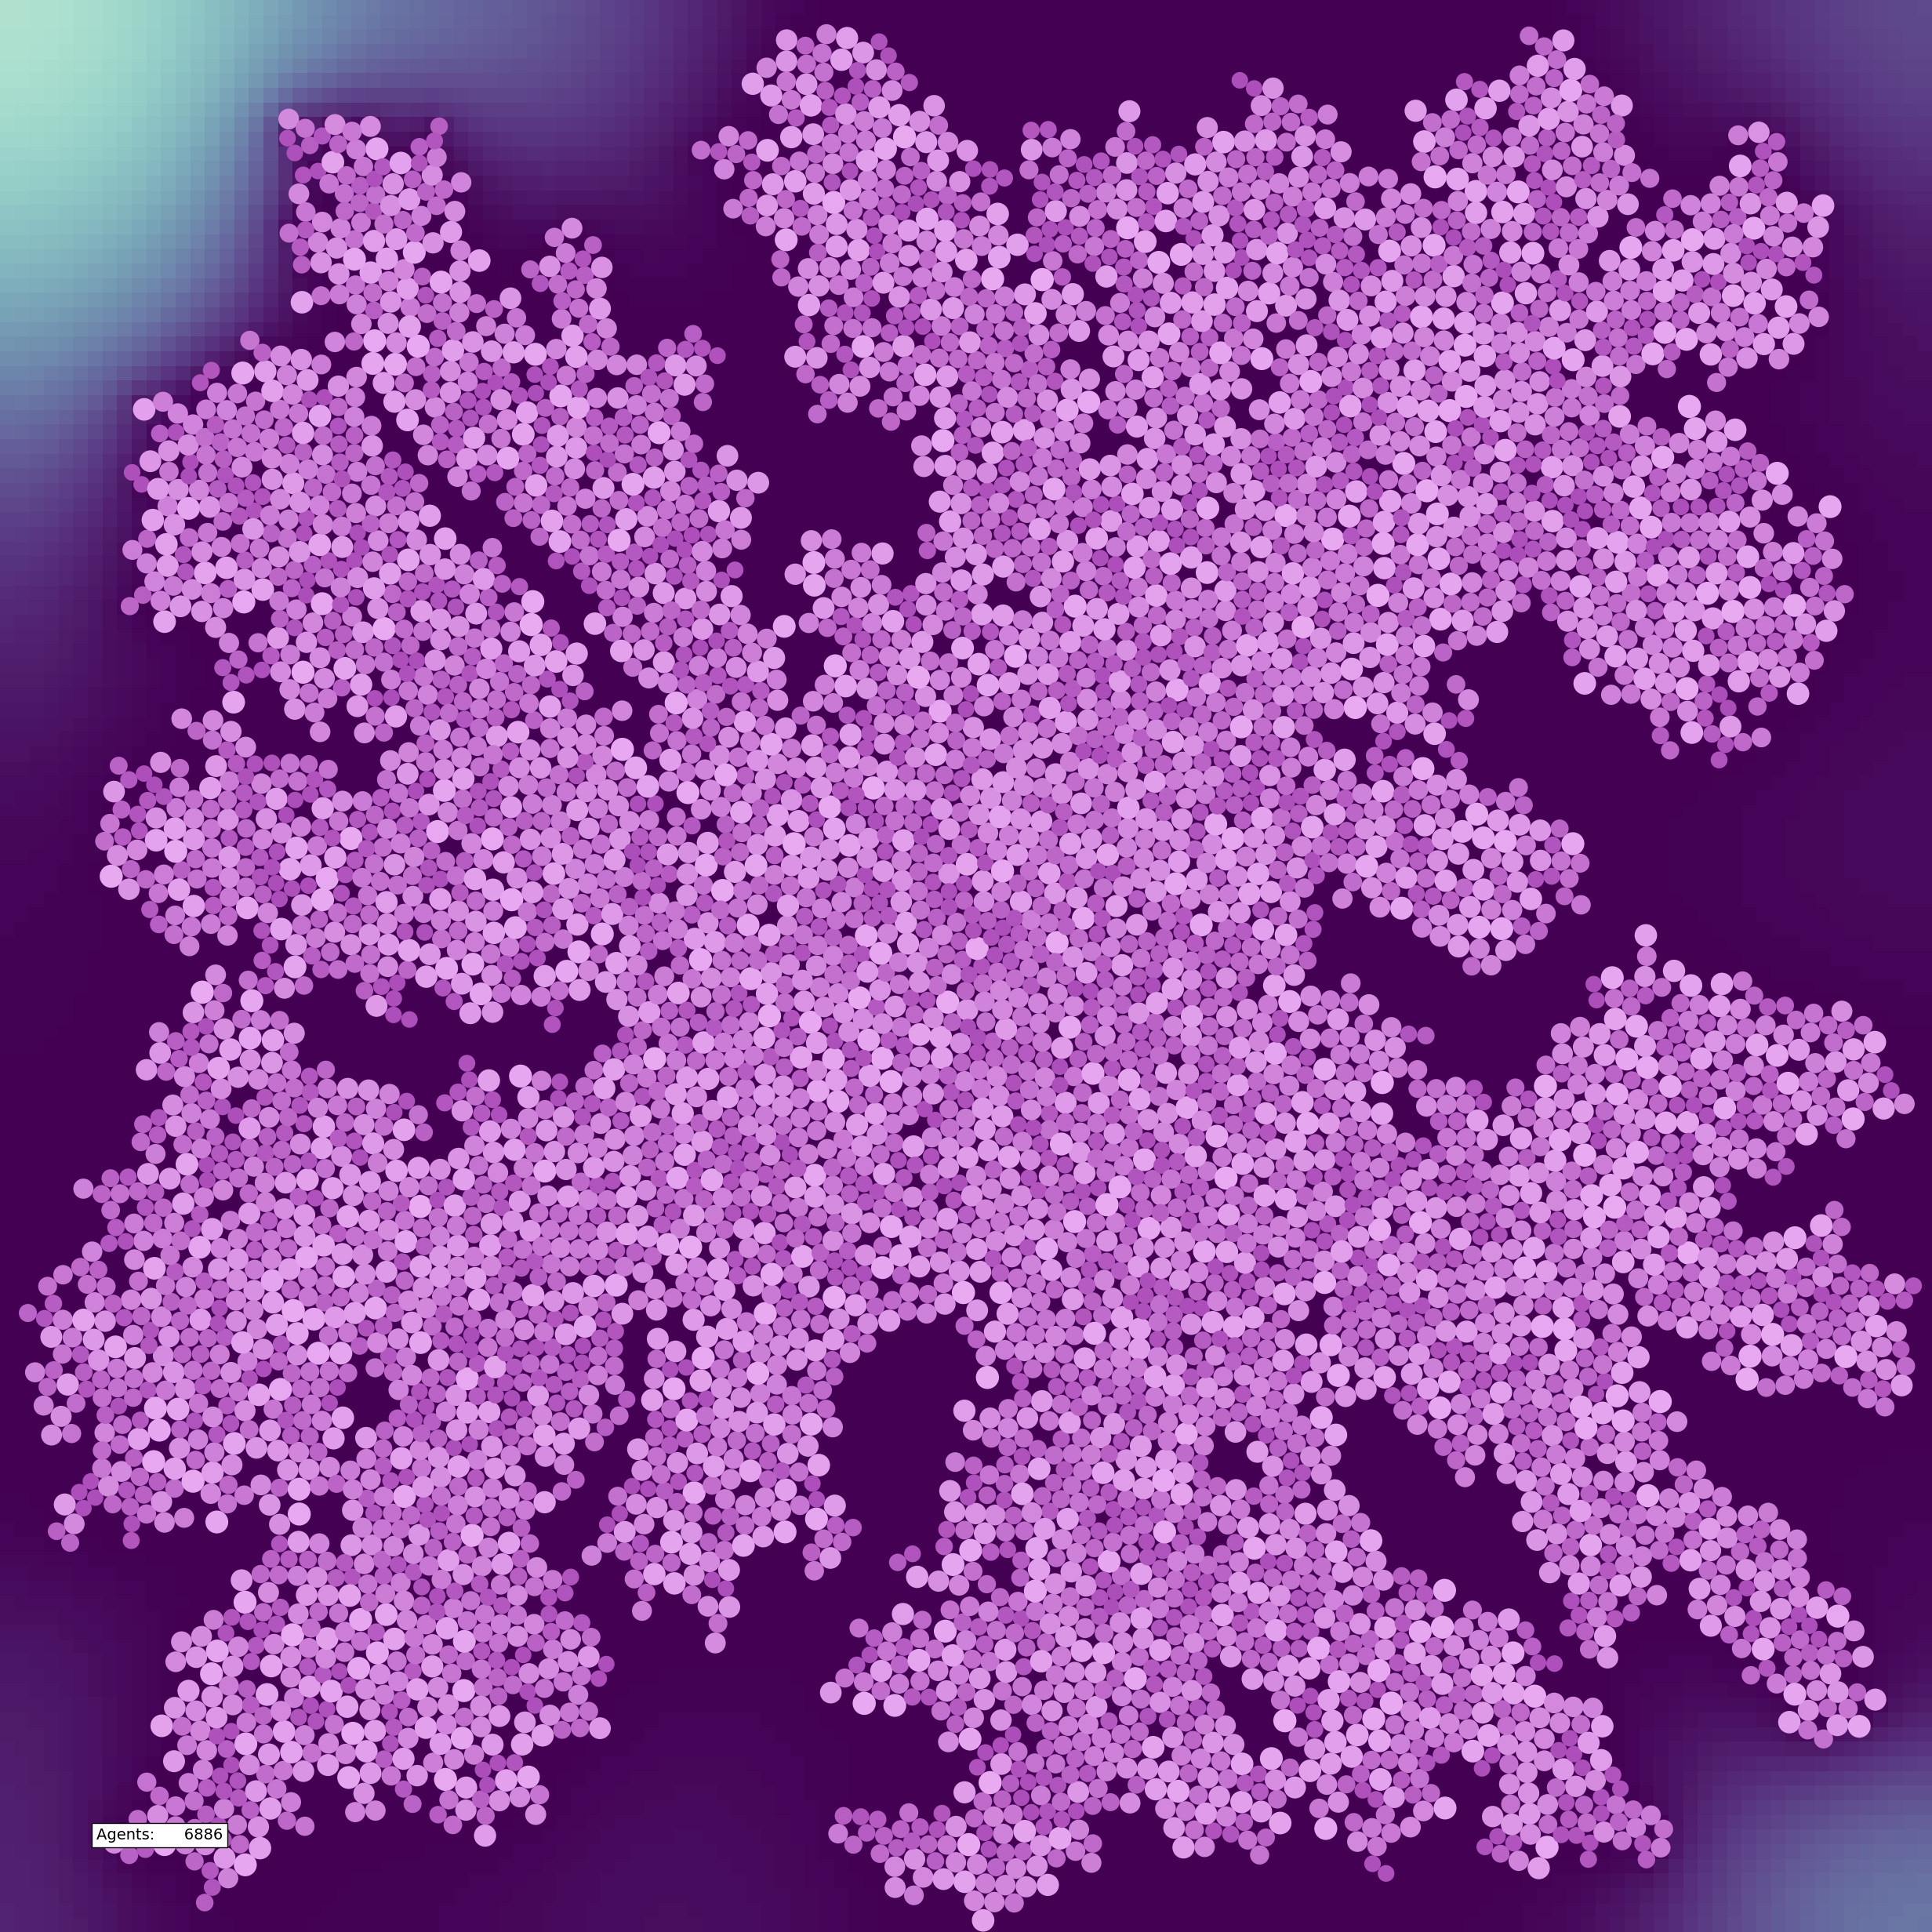
\includegraphics[width=0.49\textwidth]{figures/sim-branching/cells_at_iter_0000006600.png}%
    \hspace{0.01\textwidth}%
    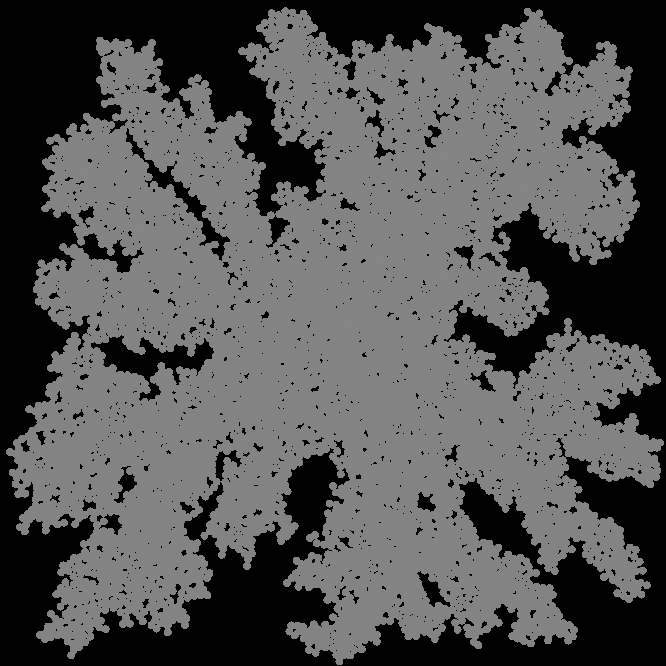
\includegraphics[width=0.49\textwidth]{figures/sim-branching/diffusion-80/discretization-nvoxels-000666.png}\\%
    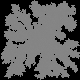
\includegraphics[width=0.49\textwidth]{figures/sim-branching/diffusion-80/discretization-nvoxels-000080.png}%
    \hspace{0.01\textwidth}%
    
\includegraphics[width=0.49\textwidth]{figures/sim-branching/diffusion-80/discretization-nvoxels-000042.png}%
    \caption{
        (A) Final simulation snapshot.
        (B-D) Coarse-graining with increasing voxel size.
    }
    \label{fig:fractal-dimension-voxel-size}
\end{figure}

\todo{include images from fractal dimension calculation}
\begin{itemize}
    \item Introduce variable $k$ which represents some type of "cutoff"
    \item everything below this cutoff is either not considered or somehow approximated by a
        coarse-grained model
    \item One can argue that all \acp{abm} live with some type of cutoff $k$ which makes it
        completely natural for not only \acp{abm} but other models as well
    \item Try to formalize how the "Running" of such a cutoff could be implemented and how the
        results could be calculated.
    \item If we consider $k$ to be spatial only, moving to a more "coarse" value will mean that
        neighbors are only interacting on their very edges of boundaries.
        This shows that coarser values of $k$ for the spatial component also allow us to consider
        coarser values for the time increment.
\end{itemize}

%###################################################################################################
\section{Other Applications}

%---------------------------------------------------------------------------------------------------
\subsection{Mechanical Properties of Rod-shaped Bacteria}
\label{subsection:bacterial-rods}

%---------------------------------------------------------------------------------------------------
\subsection{Trichome Turing Patterns on leaves of \textit{Arabidopsis Thaliana}}

% \input{ergodicity}

\bibliographystyle{IEEEtran}
\bibliography{references}

\section{Supplementary Material}
\subsection{Elementary CA}
Section~\ref{section:comparison-with-ca} formulates conditions for elementary \acp{ca} in order to
represent cellular systems.
In this section, we display results for the remaining non-trivial results for \acp{ca} that fall
under this category.
Figure~\ref{fig:supplement:ca-rules-single} shows the result of advancing a \ac{ca} from one single
living cell while Figure~\ref{fig:supplement:ca-rules-double-close} does the same for two living
cells which are separated by only one unoccupied space.

\begin{figure}[h]
    \centering
    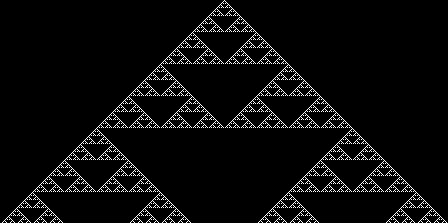
\includegraphics[width=0.32\textwidth]{ca-rules/single1/rule-018-090-146-218.pdf}%
    \hspace{0.01\textwidth}%
    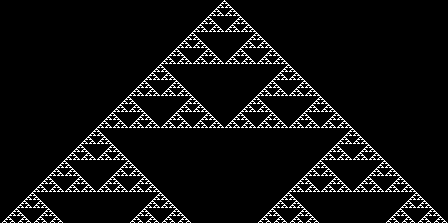
\includegraphics[width=0.32\textwidth]{ca-rules/single1/rule-022.pdf}\hspace{0.01\textwidth}%
    
\includegraphics[width=0.32\textwidth]{ca-rules/single1/rule-050-122-178-250.pdf}\\
    \vspace{0.01\textwidth}%
    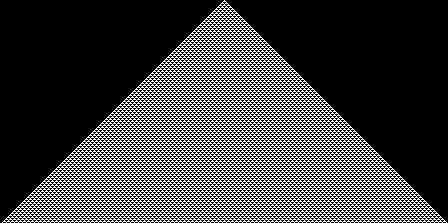
\includegraphics[width=0.32\textwidth]{ca-rules/single1/rule-054.pdf}\hspace{0.01\textwidth}%
    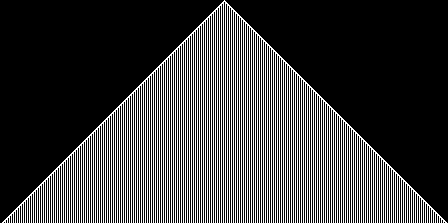
\includegraphics[width=0.32\textwidth]{ca-rules/single1/rule-094.pdf}\hspace{0.01\textwidth}%
    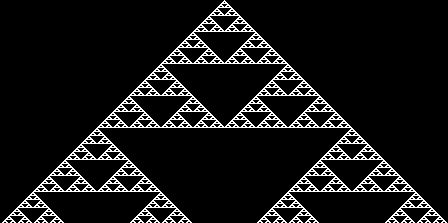
\includegraphics[width=0.32\textwidth]{ca-rules/single1/rule-126.pdf}\\
    \vspace{0.01\textwidth}
    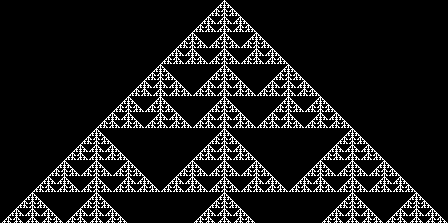
\includegraphics[width=0.32\textwidth]{ca-rules/single1/rule-150.pdf}\hspace{0.01\textwidth}%
    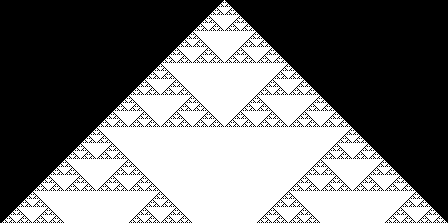
\includegraphics[width=0.32\textwidth]{ca-rules/single1/rule-182.pdf}\hspace{0.01\textwidth}%
    
\includegraphics[width=0.32\textwidth]{ca-rules/single1/rule-222-254.pdf}%
    \hspace{0.01\textwidth}%
    \caption{\todo{fill caption}}
    \label{fig:supplement:ca-rules-single}
\end{figure}

\begin{figure}[h]
    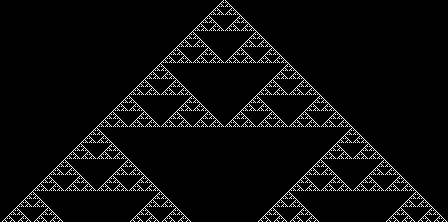
\includegraphics[width=0.32\textwidth]{ca-rules/double1-close/rule-018-090-146-218.pdf}%
    \hspace{0.01\textwidth}%
    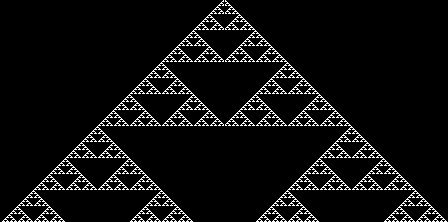
\includegraphics[width=0.32\textwidth]{ca-rules/double1-close/rule-022.pdf}%
    \hspace{0.01\textwidth}%
    
\includegraphics[width=0.32\textwidth]{ca-rules/double1-close/rule-050-122-178-250.pdf}\\%
    \vspace{0.01\textwidth}%
    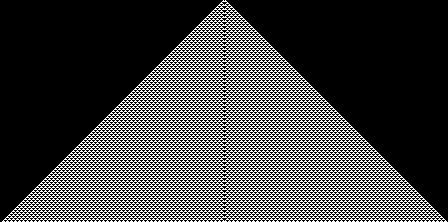
\includegraphics[width=0.32\textwidth]{ca-rules/double1-close/rule-054.pdf}%
    \hspace{0.01\textwidth}%
    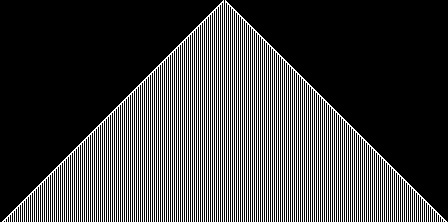
\includegraphics[width=0.32\textwidth]{ca-rules/double1-close/rule-094.pdf}%
    \hspace{0.01\textwidth}%
    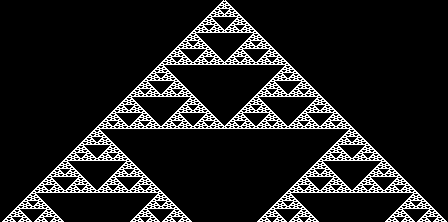
\includegraphics[width=0.32\textwidth]{ca-rules/double1-close/rule-126.pdf}\\%
    \vspace{0.01\textwidth}%
    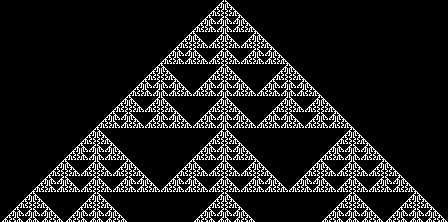
\includegraphics[width=0.32\textwidth]{ca-rules/double1-close/rule-150.pdf}%
    \hspace{0.01\textwidth}%
    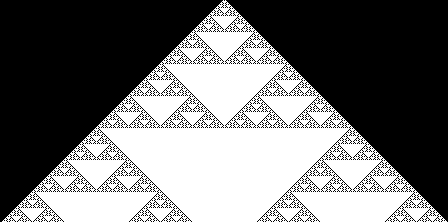
\includegraphics[width=0.32\textwidth]{ca-rules/double1-close/rule-182.pdf}\\%
    \vspace{0.01\textwidth}%
    
\includegraphics[width=0.32\textwidth]{ca-rules/double1-close/rule-222.pdf}%
    \hspace{0.01\textwidth}%
    
\includegraphics[width=0.32\textwidth]{ca-rules/double1-close/rule-254.pdf}%
    \hspace{0.01\textwidth}%
    \caption{\todo{fill caption}}
    \label{fig:supplement:ca-rules-double-close}
\end{figure}
